%
% Complete documentation on the extended LaTeX markup used for Insight
% documentation is available in ``Documenting Insight'', which is part
% of the standard documentation for Insight.  It may be found online
% at:
%
%     http://www.itk.org/

\documentclass{InsightArticle}

\usepackage[dvips]{graphicx}



%%%%%%%%%%%%%%%%%%%%%%%%%%%%%%%%%%%%%%%%%%%%%%%%%%%%%%%%%%%%%%%%%%
%
%  hyperref should be the last package to be loaded.
%
%%%%%%%%%%%%%%%%%%%%%%%%%%%%%%%%%%%%%%%%%%%%%%%%%%%%%%%%%%%%%%%%%%
\usepackage[dvips,
bookmarks,
bookmarksopen,
backref,
colorlinks,linkcolor={blue},citecolor={blue},urlcolor={blue},
]{hyperref}

\usepackage{url}


%  This is a template for Papers to the Insight Journal. 
%  It is comparable to a technical report format.

% The title should be descriptive enough for people to be able to find
% the relevant document.
\title{CTest Integration of Sikuli Automated GUI Testing}

% 
% NOTE: This is the last number of the "handle" URL that 
% The Insight Journal assigns to your paper as part of the
% submission process. Please replace the number "1338" with
% the actual handle number that you get assigned.
%
\newcommand{\IJhandlerIDnumber}{3196}

% Increment the release number whenever significant changes are made.
% The author and/or editor can define 'significant' however they like.
\release{0.00}

% At minimum, give your name and an email address.  You can include a
% snail-mail address if you like.
\author{Evan Schwab, Arnaud Gelas, Lydie Souhait, Nicolas Rannou,\\
Kishore Mosaliganti, Sean Megason}
\authoraddress{Megason Lab, Department of Systems Biology, Harvard Medical
School}

\begin{document}

% Add hyperlink to the web location and license of the paper.
\IJhandlefooter{\IJhandlerIDnumber}


\ifpdf
\else
   %
   % Commands for including Graphics when using latex
   %
   \DeclareGraphicsExtensions{.eps,.jpg,.gif,.tiff,.bmp,.png}
   \DeclareGraphicsRule{.jpg}{eps}{.jpg.bb}{`convert #1 eps:-}
   \DeclareGraphicsRule{.gif}{eps}{.gif.bb}{`convert #1 eps:-}
   \DeclareGraphicsRule{.tiff}{eps}{.tiff.bb}{`convert #1 eps:-}
   \DeclareGraphicsRule{.bmp}{eps}{.bmp.bb}{`convert #1 eps:-}
   \DeclareGraphicsRule{.png}{eps}{.png.bb}{`convert #1 eps:-}
\fi

\maketitle

\ifhtml
\chapter*{Front Matter\label{front}}
\fi

\begin{abstract}
\noindent
 
\end{abstract}

\IJhandlenote{\IJhandlerIDnumber}

\tableofcontents
% ------------------------------------------------------------------------
\section{Introduction}

%Should this be in the abstract instead?
% difference between Abstract and Introduction?

GUI testing is a key aspect of software development. Having a well defined
testing protocol is very important in maintaining a productive flow, especially
on the eve of a new release. As the software becomes more complex, testing each
feature can be immensely time consuming. We collected a list of over 400
different GUI tests for the GoFigure2 software~\cite{GoFigure2:Website} which
involved endlessly repetitive clicking and checking. This task took around 5
hours to complete each time a new release was ready. And debugging would push
release dates back days or even weeks. We decided to tackle this problem by
utilizing a new scripting language called
Sikuli~\cite{Sikuli:Documentation,Sikuli:Website,Yeh:2009:Sikuli} that can
automate any visual operation. In this way we could write scripts to automate
the GUI testing. This cut the time to complete each test drastically.
Furthermore, we have integrated the automated tests with CTest. Therefore we
are able to run the collection of tests every night and find bugs as they
arise instead of the night before a new release. As a result, the rate of new
releases increased drastically.\\

The paper is organized as follows, first we will briefly introduce what is
Sikuli (in section~\ref{sec:WhatIsSikuli}) and show one simple example (in
section~\ref{sec:SimpleSikuliExample}). Then we will show a real test example
on GoFigure2 (in section~\ref{sec:GoFigure2Example}) and how to integrate
unit tests in CTest (in section~\ref{sec:IntegrationWithCTest}). Finally, we
will review the current limitation of Sikuli and this approach for GUI Testing
(in section~\ref{sec:Limitations}) and conclude (in
section~\ref{sec:Conclusion}).

% Should the intro be about GoFigure2? with picture of GoFigure2
% Also consult actual number of tests.
%See Figure 3 ? -- picture of GIT log from presentation

% ------------------------------------------------------------------------
\section{Sikuli}

% Feel free to change section titles
\subsection{What is Sikuli?}
\label{sec:WhatIsSikuli}

Sikuli~\cite{Sikuli:Documentation,Sikuli:Website,Yeh:2009:Sikuli} is a visual
technology to automate and test graphical user interfaces (GUI) using images
(screenshots). Sikuli includes \emph{Sikuli Script} and \emph{Sikuli IDE}.\\

\emph{Sikuli Script} automates anything you see on the screen without internal
API's support. Sikuli Script is a programming language that uses screenshot
images as variables and objects in order to automate graphical user interface
functions. The Sikuli Script is built on a Jython (Python for Java platform)
library which uses Python syntax in addition to a number of special Sikuli
functions for acquiring and handling screenshot images and performing mouse,
keyboard actions.\\

In the \emph{Sikuli IDE}, the user can write scripts that include screenshot
thumbnails so they can visually track the functions of their code. The most
useful functions from Sikuli scripts are conveniently found as
buttons on the IDE. When using the IDE, Sikuli then saves a script in a
directory with a unique extension .sikuli. The directory consists of a python
script file (script file to be used by sikuli), an html file, and a list of all
the screenshot images used in the script.

% ------------------------------------------------------------------------
\subsection{Simple Sikuli example} % not related to gofigure...
\label{sec:SimpleSikuliExample}

Figure~\ref{fig:SimpleExample} shows the Sikuli-IDE for version 0.10.2. On the
left-hand side menu is a list of commonly used Sikuli commands
like \emph{find}(), \emph{click}(), and \emph{type}(). The picture of
the camera within the parentheses indicates the screenshot input variable.
Clicking on any of these menu functions will automatically set up the Sikuli
screenshot mode, whereby the Sikuli-IDE disappears and what is on the screen at
that moment is available to capture by selecting a rectangular region of
interest. The function will then appear in the scripting domain with the snap
shot in parentheses as shown in Figure~\ref{fig:SimpleExample}. The user may
also type in the function and invoke the screenshot mode by clicking on the
camera in the top menu or by using a keyboard shortcut. The simple Sikuli script
example in Figure~\ref{fig:SimpleExample} will open gedit Text Editor, type a
message, and save the file.

\begin{figure}[tbp]
 \centering
 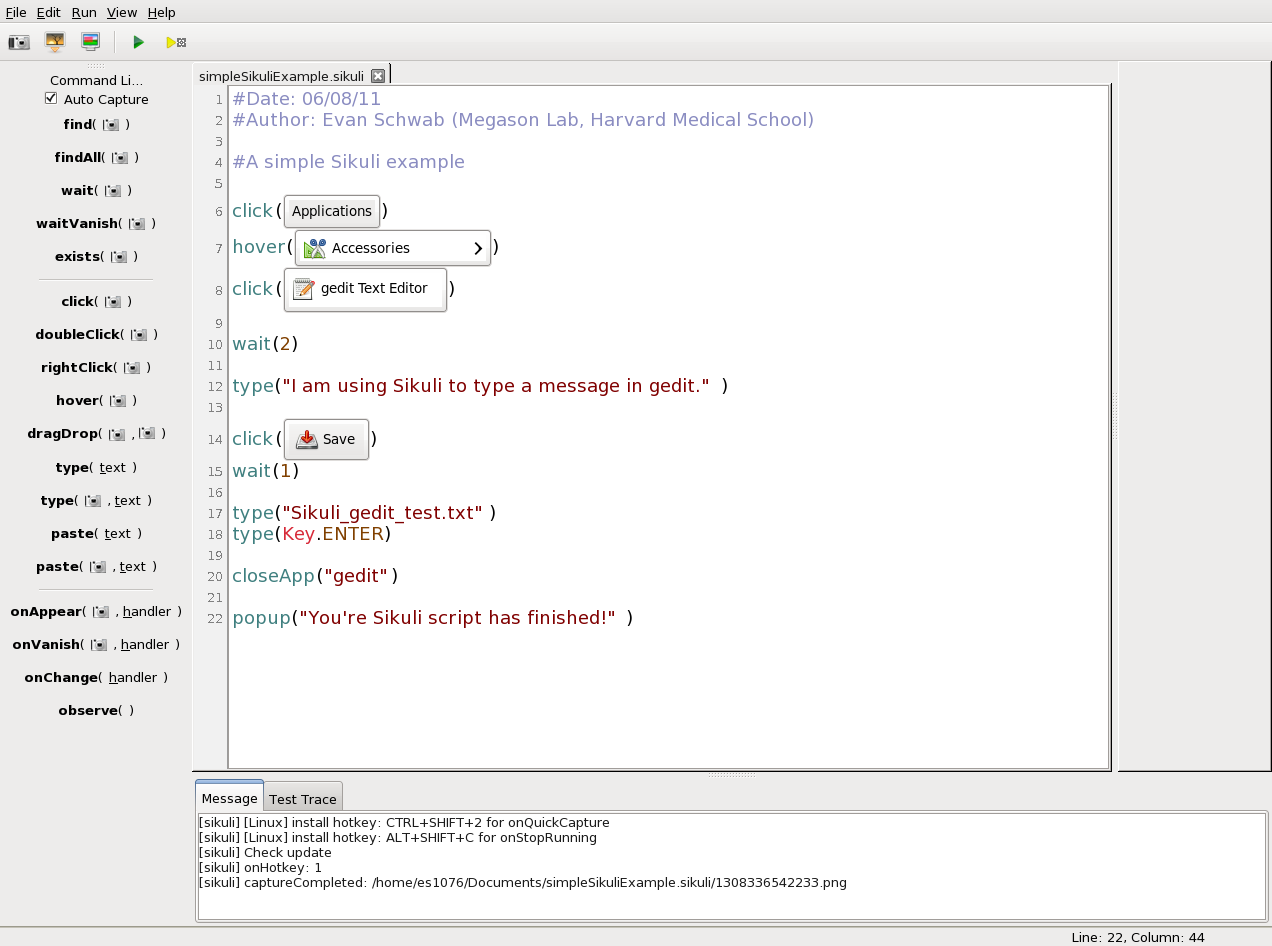
\includegraphics[width=0.99\textwidth]{Images/SimpleSikuliExample.png}
 % SimpleSikuliExample.png: 1280x1024 pixel, 72dpi, 45.16x36.12 cm, bb=0 0 1280 1024
 \caption{Simple Sikuli Script Example in Sikuli-IDE}
 \label{fig:SimpleExample}
\end{figure}

% ------------------------------------------------------------------------
\section{Example}
\label{sec:GoFigure2Example}

The GoFigure2 software~\cite{GoFigure2:Website} (See
Figure~\ref{fig:GoFigure2GUI}) is designed to automate
cell segmentation and tracking for high resolution microscopy data and the
Megason Lab uses it to create cell lineages of developing zebrafish emrbryos.
The Sikuli script in Figure~\ref{fig:Gofigure2Example} shows a fragment of a
unit test for our GoFigure2 software. The unit being tested here is the Toolbar
menu which consists of different modes used to analyze data set plots. In total
there are four modes which are represented in the first line as the vector
Toolbar and for each of these modes we want to test their expected
mouse functions. For instance, if we are in the zoom Toolbar mode then we want
the data set plot to zoom in when the user scrolls the mouse wheel
forward. Likewise, if we are in pan mode then we want the plot to move to the
left if the user holds down the left mouse button and moves the mouse to
the left. Also importantly, we want to see that these two mouse actions are
unique for their respective Toolbar modes; the test will include an assertion
that scrolling forward will zoom in when using zoom mode and will do nothing
when using pan mode.\\

\begin{figure}[tbp]
 \centering
 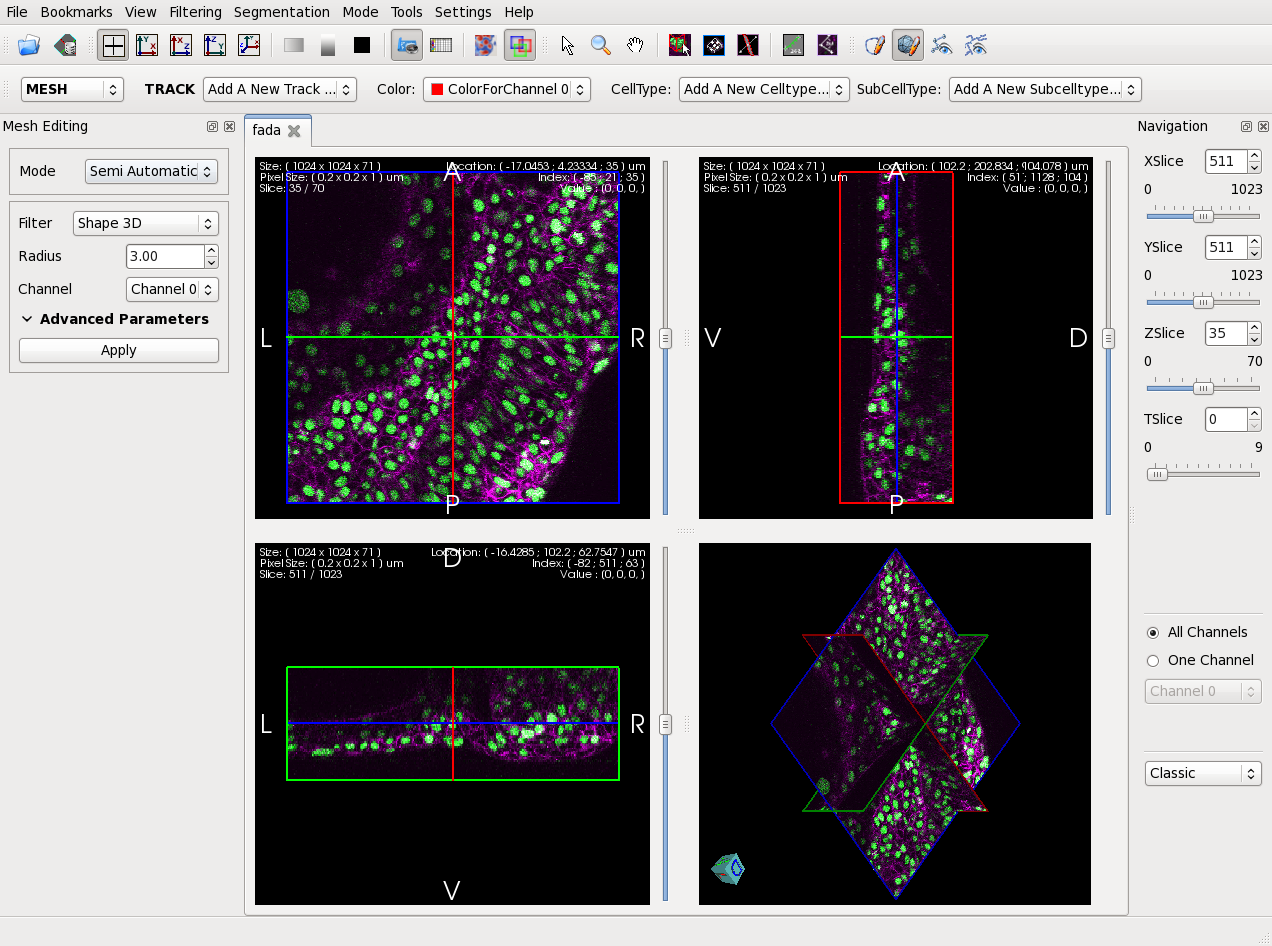
\includegraphics[width=0.99\textwidth]{Images/Gofigure2GUI.png}
 % SimpleSikuliExample.png: 1280x1024 pixel, 72dpi, 45.16x36.12 cm, bb=0 0 1280
 \caption{GoFigure2 GUI Interface}
 \label{fig:GoFigure2GUI}
\end{figure}


This breakdown of modes and actions lends itself to a nested for-loop scripting
approach. By representing these variables as a vector the software developers
can easily add new modes or actions to each list to be tested, when the software
is updated. Similarly, the tester can easily replace any of the screenshot
images with images of updated GUI icons.\\  

In addition to representing the modes and actions as the vectors Toolbar and
Mouse, respectively, we have included the different data set plots in the
vector ViewRegion. These images represent the \emph{xy-}, \emph{xz-},
\emph{yz-}, and \emph{xyz-}views of zebrafish microscopy data taken in the
Megason Lab. After capturing these images we can then use them to locate their
initial pixel coordinates within the GoFigure2 GUI using the \emph{find}()
function. These points become our reference positions to calculate directional
movement.  For example, when testing the pan mode, we mark the initial position
of each image, use the \emph{mouseMove}() function to a chosen location, and
then use \emph{find}() to obtain the new coordinates. We can then assert if the
image panned as it should have. Similarly for zoom, we can first find the area
of the image and then find the area of the zoomed in image.  To test the result
when the user clicks in a certain mode, we've made use of Sikuli's \emph{assert
exists}() function to ascertain the existence of our desired results (see
Figure~\ref{fig:Gofigure2Example}).\\

This one GUI test is then combined with other GoFigure2 tests in succession and
the Sikuli Unit Testing CTest integration will identify which tests pass and
which fail and when. Many of the units need to be tested in a certain order.
For example, in order to test the Toolbar modes on the data sets, one first
needs to test the software's data import functionality.

\begin{figure}[tbp]
 \centering
 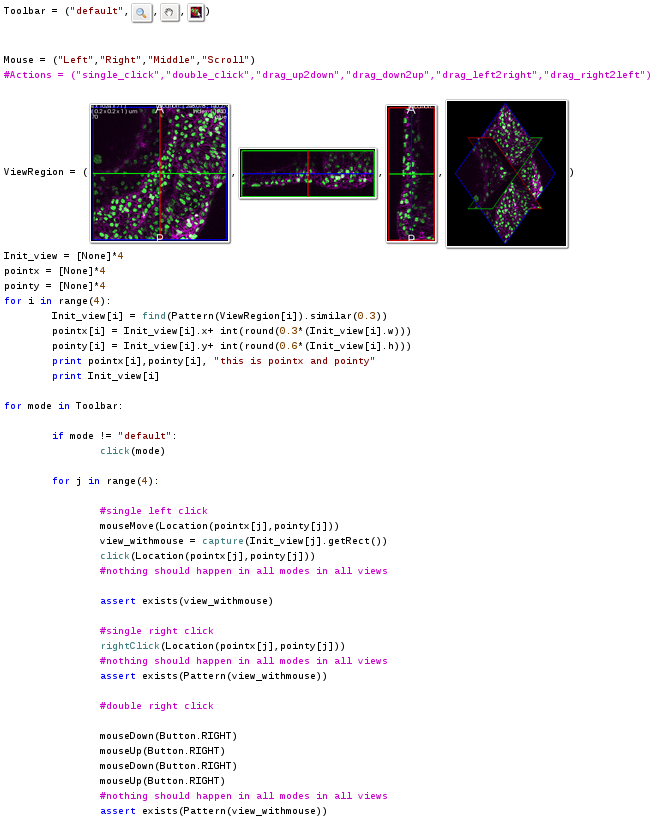
\includegraphics[width=0.99\textwidth]{Images/Gofigure2Example.png}
 % Gofigure2Example.png: 667x826 pixel, 72dpi, 23.53x29.14 cm, bb=0 0 667 826
 \caption{Sikuli Script for Gofigure2 GUI Testing}
 \label{fig:Gofigure2Example}
\end{figure}

% ------------------------------------------------------------------------
\section{Integration with CTest}
\label{sec:IntegrationWithCTest}

\subsection{CMake}

One of Sikuli's primary uses is the automation of GUI testing for software
developers. For GUI testing, it is useful to compartmentalize different software
functions and test each unit individually.\\

The newest versions of Sikuli come equipped with a Unit Testing feature based
on JUnit~\cite{JUnit:Website}. Unit Testing can be called using the IDE or by
command line and enables the user to write multiple functions in a script which
are run individually. At the end of the run, the Sikuli output will tell the
user how many tests ran successfully and which ones failed and where.\\

Here we connect this Unit Testing feature to CTest, which allows us to report
results on a public dashboard using CDash. To this end, we developed cmake
functions to discover where Sikuli is installed and special functions to add
Sikuli tests in the list for CTest.

Here is a typical CMakeLists.txt file, to be able to use such functionalities:

\begin{verbatim}
# first let's include CTest and enable testing

include( CTest )
enable_testing()

# Then let's
#   - figure out where Sikuli is installed
#   - define function to add Sikuli tests

find_package( Sikuli )

# here we add a sikuli test
add_sikuli_test( GoFigure2ToolbarTest toolbar.sikuli )
\end{verbatim}

Users can either maintain an image library or keep images in the
corresponding Sikuli script directory (default). If one uses an image library,
the corresponding path must be set during CMake time in
the SIKULI\_IMAGE\_LIBRARY\_DIR variable.

\subsection{Unit Test Script Format}

Unit testing scripts are written as a series of functions defined by pythons
keyword def.  The constructing and destructing methods,
\emph{setUp}() and \emph{tearDown}(), are used to start and end the software
GUI and methods in between are named with the prefix test.

\begin{verbatim}
def setUp(self):
  print "setUp";

def testPrint(self):
  print "dummy test to validate, it is printing on the screen!";

def tearDown(self):
  print "tearDown";
\end{verbatim}

When this script is run with the Sikuli Unit Testing feature, it will report the
results of each test method in CTest and then reported automatically on
CDash.

% ------------------------------------------------------------------------
\section{Current Limitations}
\label{sec:Limitations}

Sikuli's integration with CTest has provided us with numerous advantages in the
measure of productivity and convenience. But our goals are still
hindered by a few limitations.

%\subsection{Text Recognition}
%Sikuli's newer versions come equipped with a text recognition feature whereby
%one can search for a string of text instead of searching for the image of the
%text in the GUI.  This makes programming in Sikuli much simpler but it is
%limited by it's searchable text fonts.

\subsection{Off-screen Rendering}

Our goal in using CTest is that we will be able to test our software 
automatically every night and bugs can be reported the next day on CDash. 
But Sikuli is not easily compatible with off-screen rendering. Sikuli 
requires that the screen remains on so that the script can identify the 
images on the screen. In addition, external mouse and keyboard actions can 
disrupt the script at any moment. These factors make it more difficult to 
set up automated nightly tests.

\subsection{Variation of style between machines}

Another important issue is the difference between operating systems.
Developers need to make sure that their software runs on each OS. But
Different operating systems require different libraries for generating GUI
images. Therefore fonts, icons, and even layouts will differ between
machines. This is also true between versions of the same OS. So, GUI tests
that pass on one machine will inevitably fail on another machine for the
same exact software. This requires developers to write the same Sikuli 
script using images from each OS, which will be many times the workload.

\subsection{CDash}
Furthermore, CDash does not currently support Sikuli script since images used
in the script are unable to be displayed on the dashboard.  Without these
images on CDash, visualize which units are being tested.  In addition, CDash
does not make the distinction between simple syntax errors versus a complete
test failure. These are
extensions to CDash that can be corrected for future work.

% ------------------------------------------------------------------------
\section{Conclusion}
\label{sec:Conclusion}

\clearpage

\bibliographystyle{plain}
\bibliography{InsightJournal,biblio}


\end{document}

